\chapter{Multi view terrestrial laser scan registration}

\begin{figure}
	\centering
	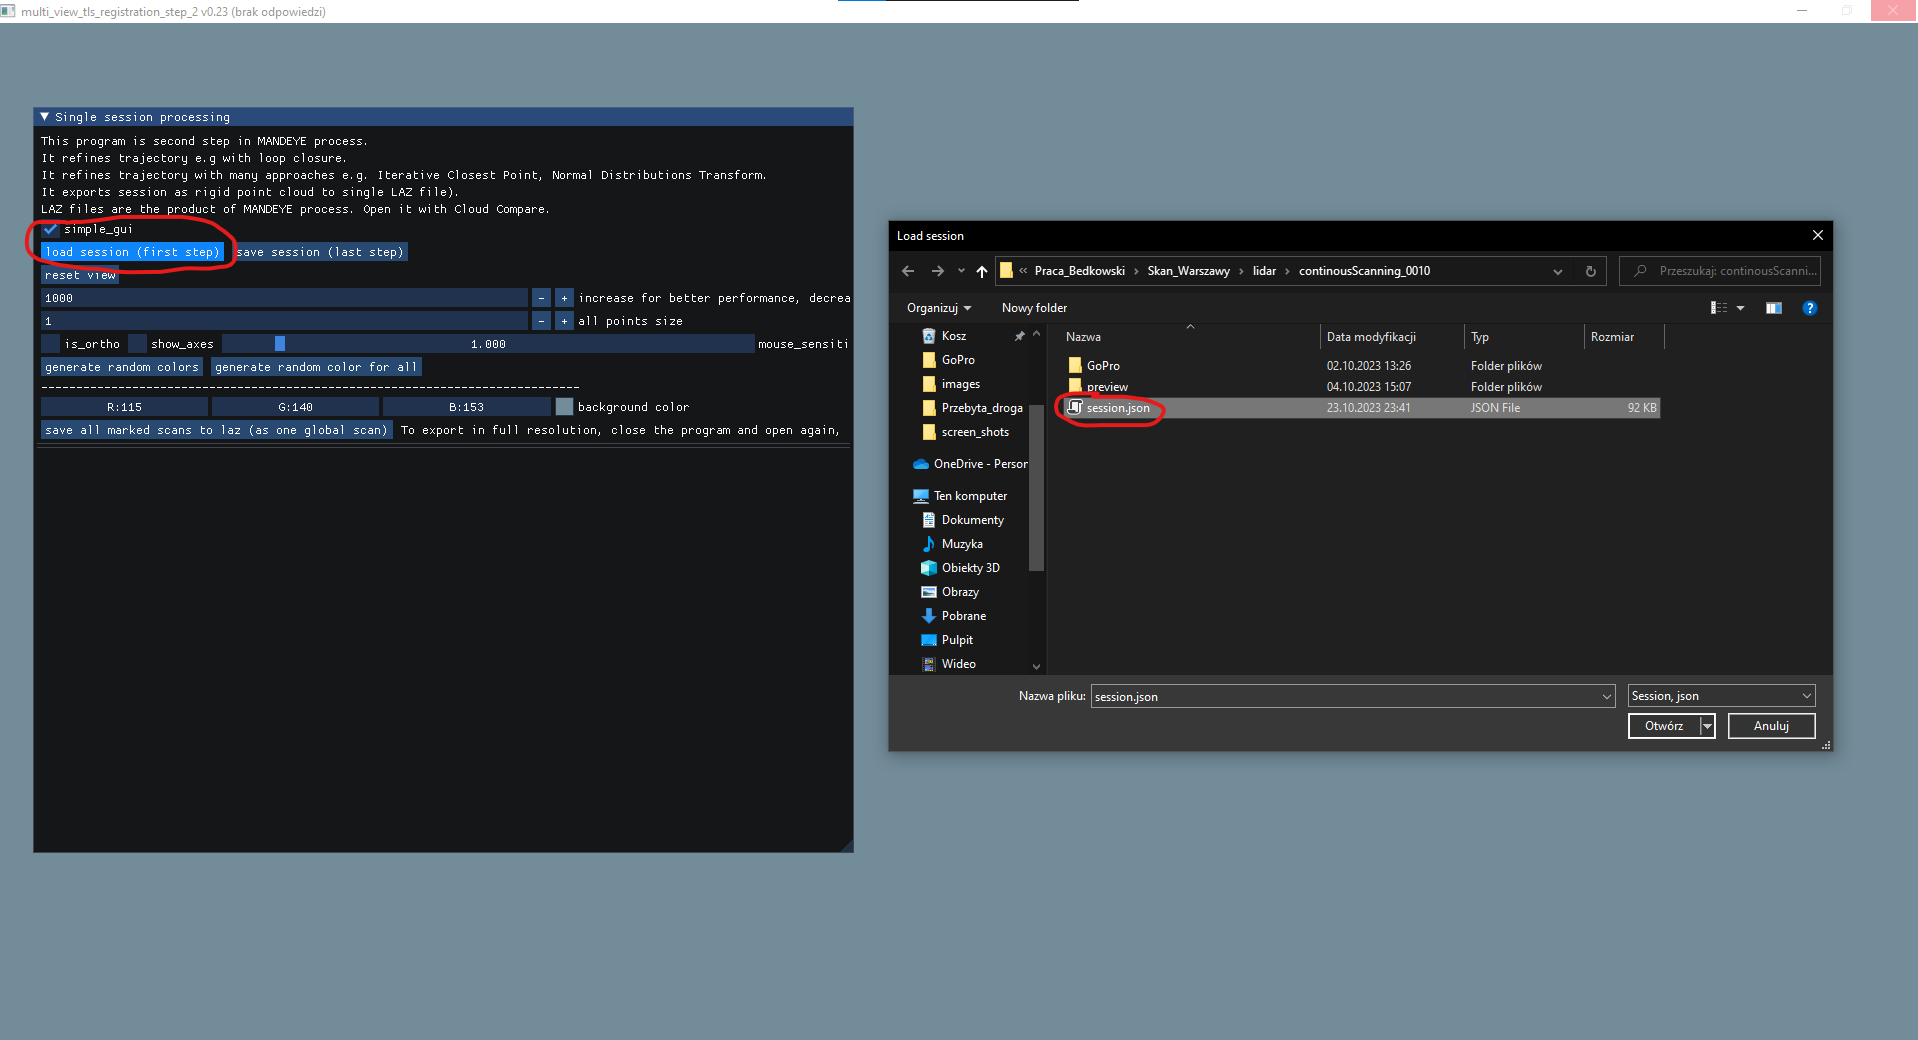
\includegraphics[width=\textwidth]{10.png}
	\caption{Import files prepared by 'Lidar odometry'.}
	\label{fig:10}
\end{figure}

\begin{figure}
	\centering
	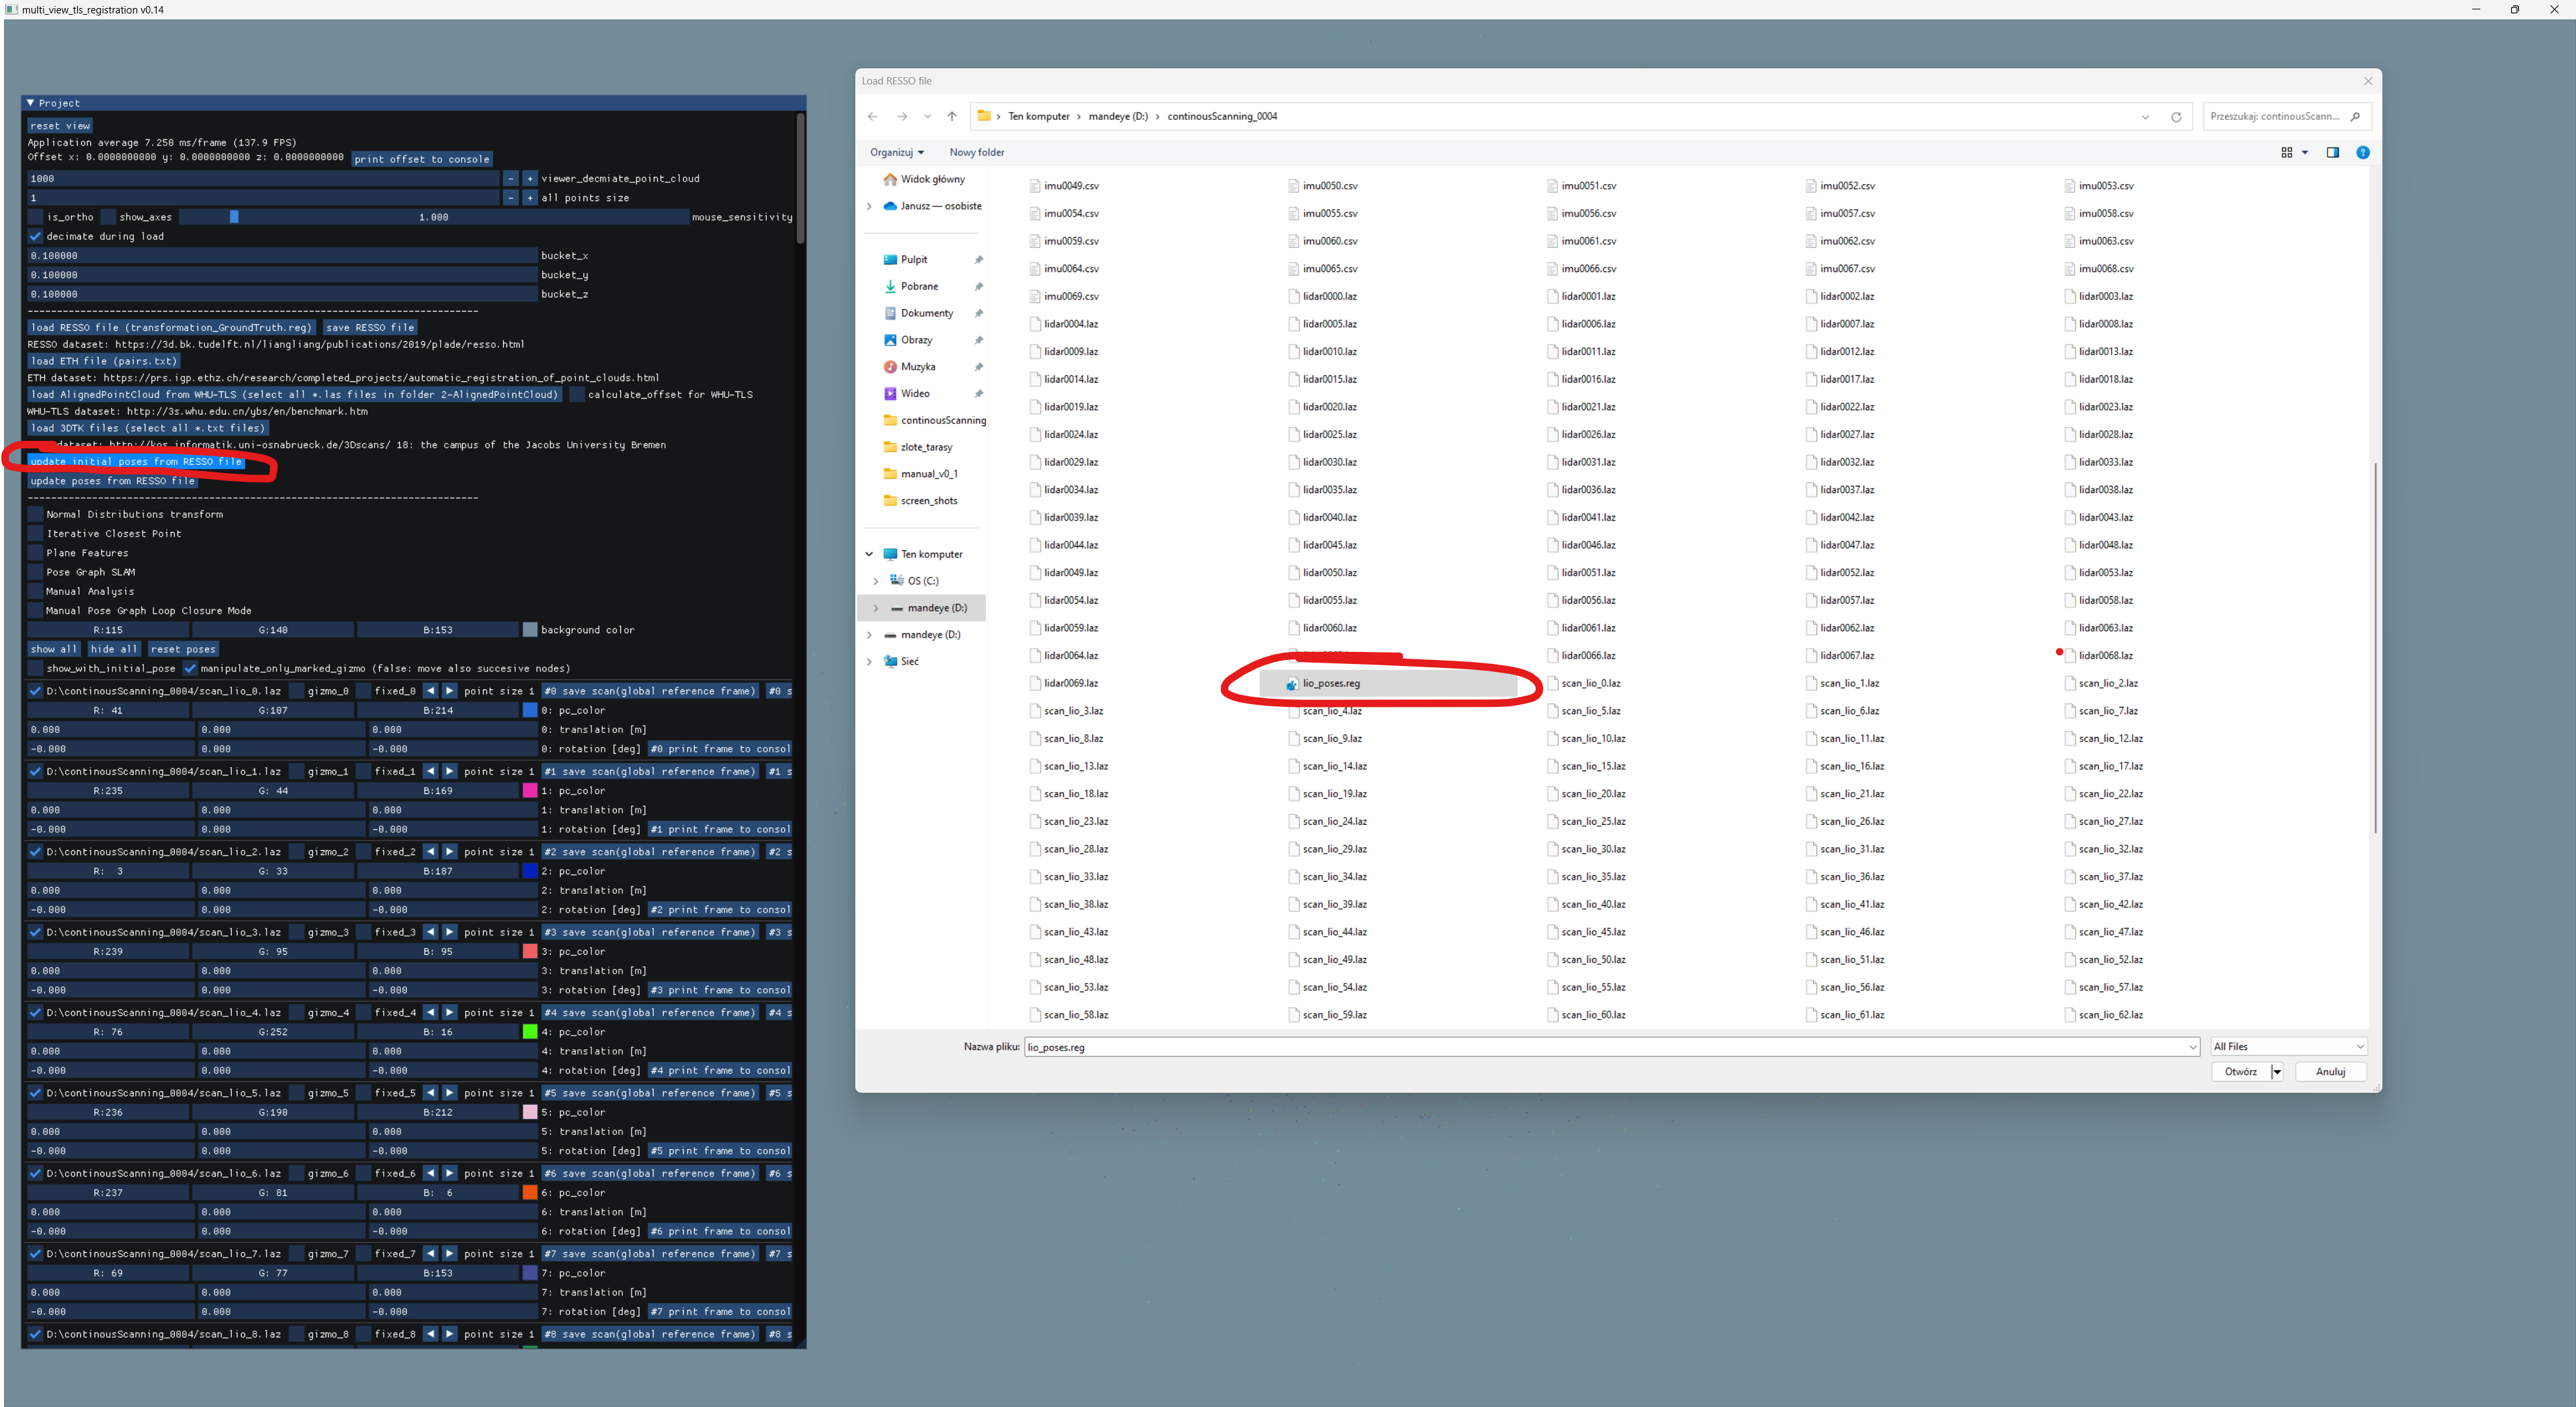
\includegraphics[width=\textwidth]{11.png}
	\caption{Update initial poses from *.reg file.}
	\label{fig:11}
\end{figure}


\begin{figure}
	\centering
	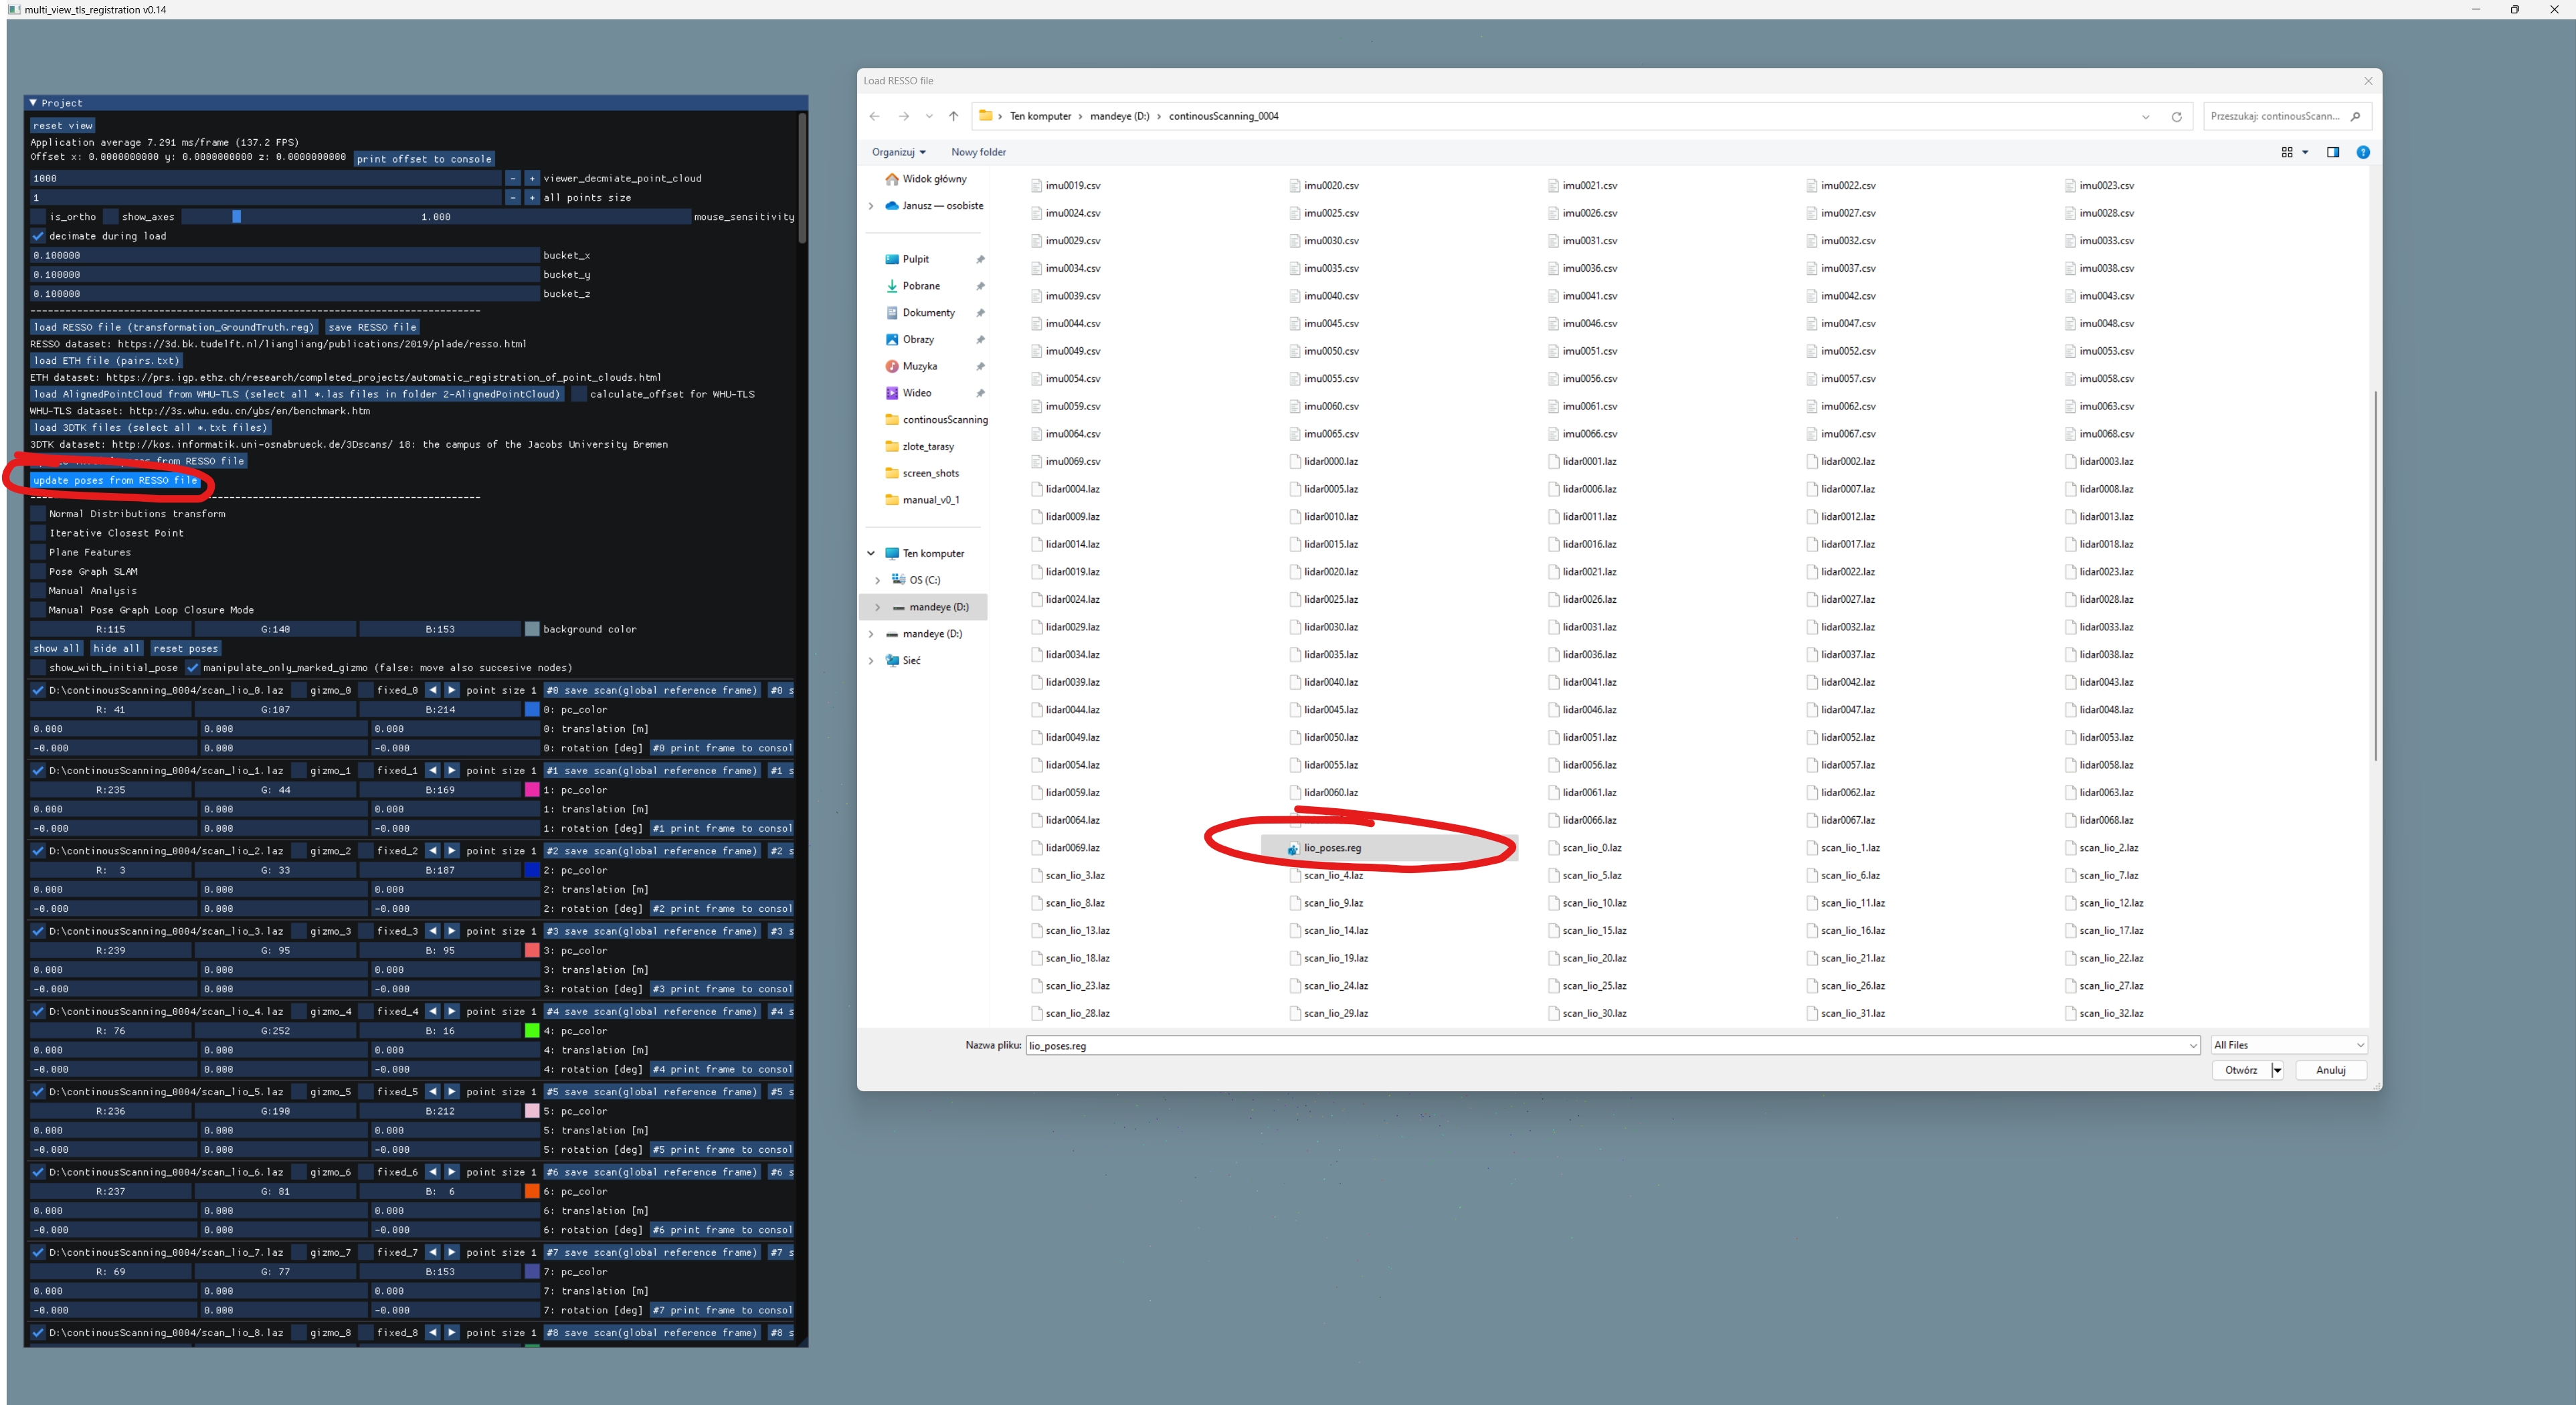
\includegraphics[width=\textwidth]{12.png}
	\caption{Update poses from *.reg file.}
	\label{fig:12}
\end{figure}

\begin{figure}
	\centering
	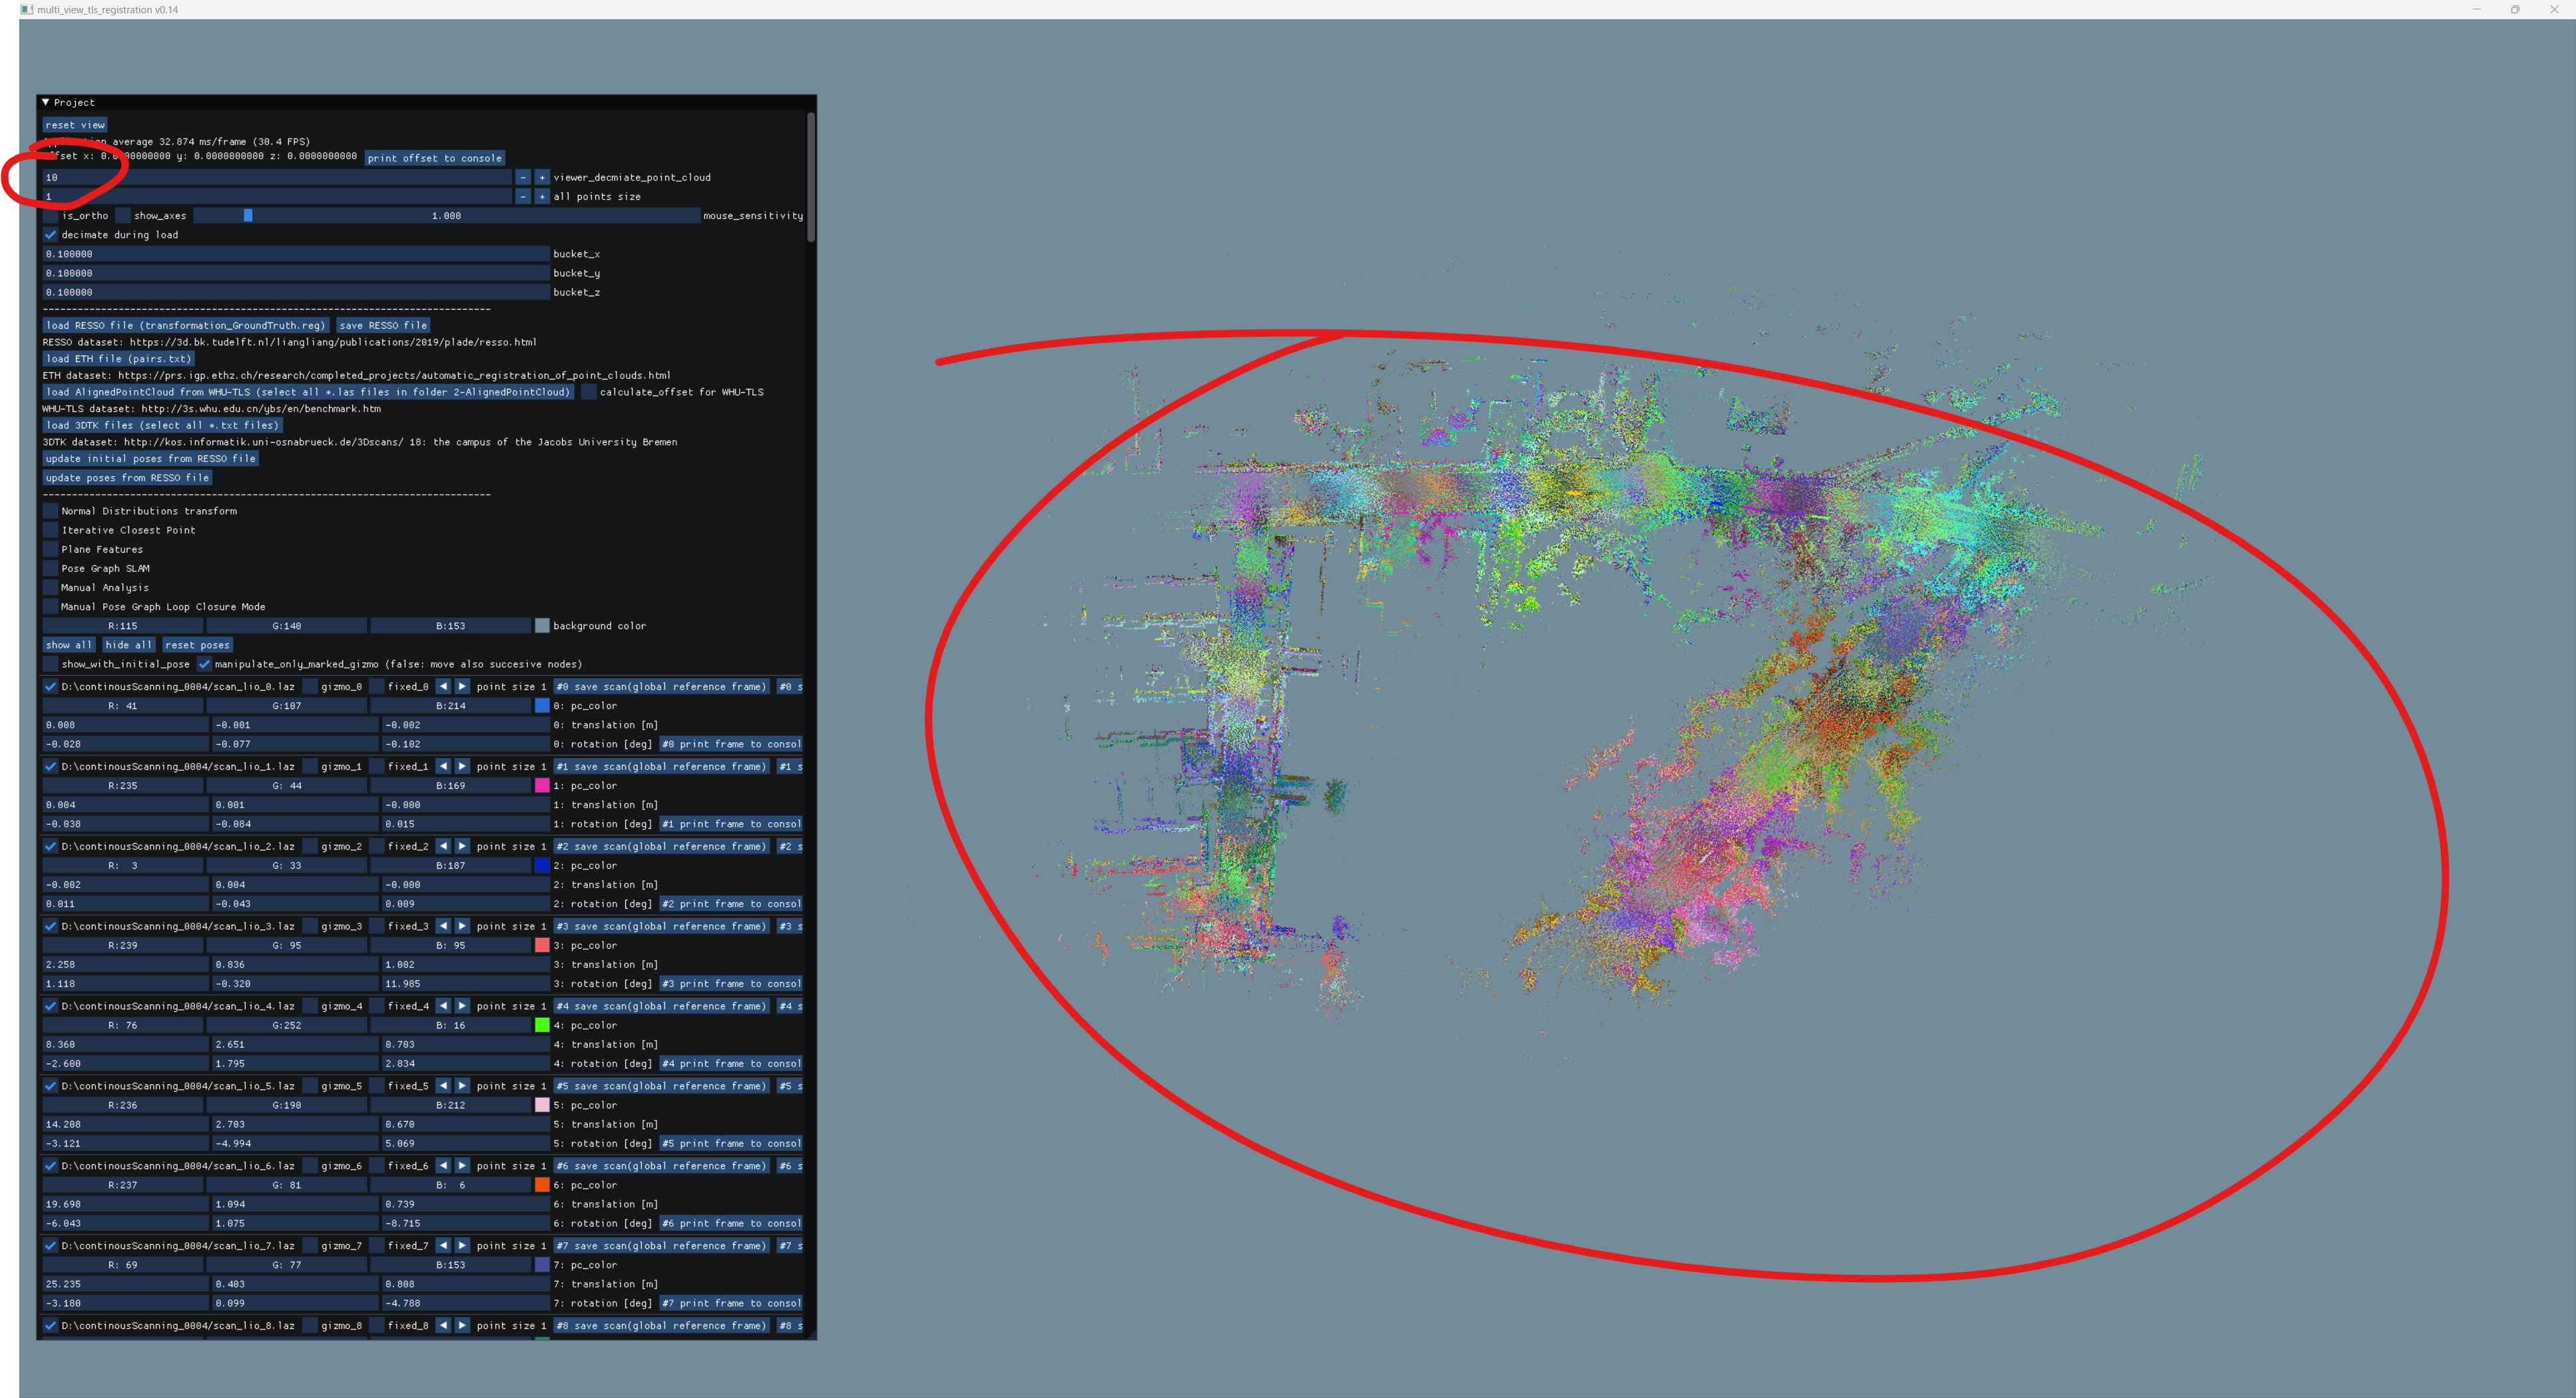
\includegraphics[width=\textwidth]{13.png}
	\caption{Prepare field of view and change decimation to see more points.}
	\label{fig:13}
\end{figure}

\begin{figure}
	\centering
	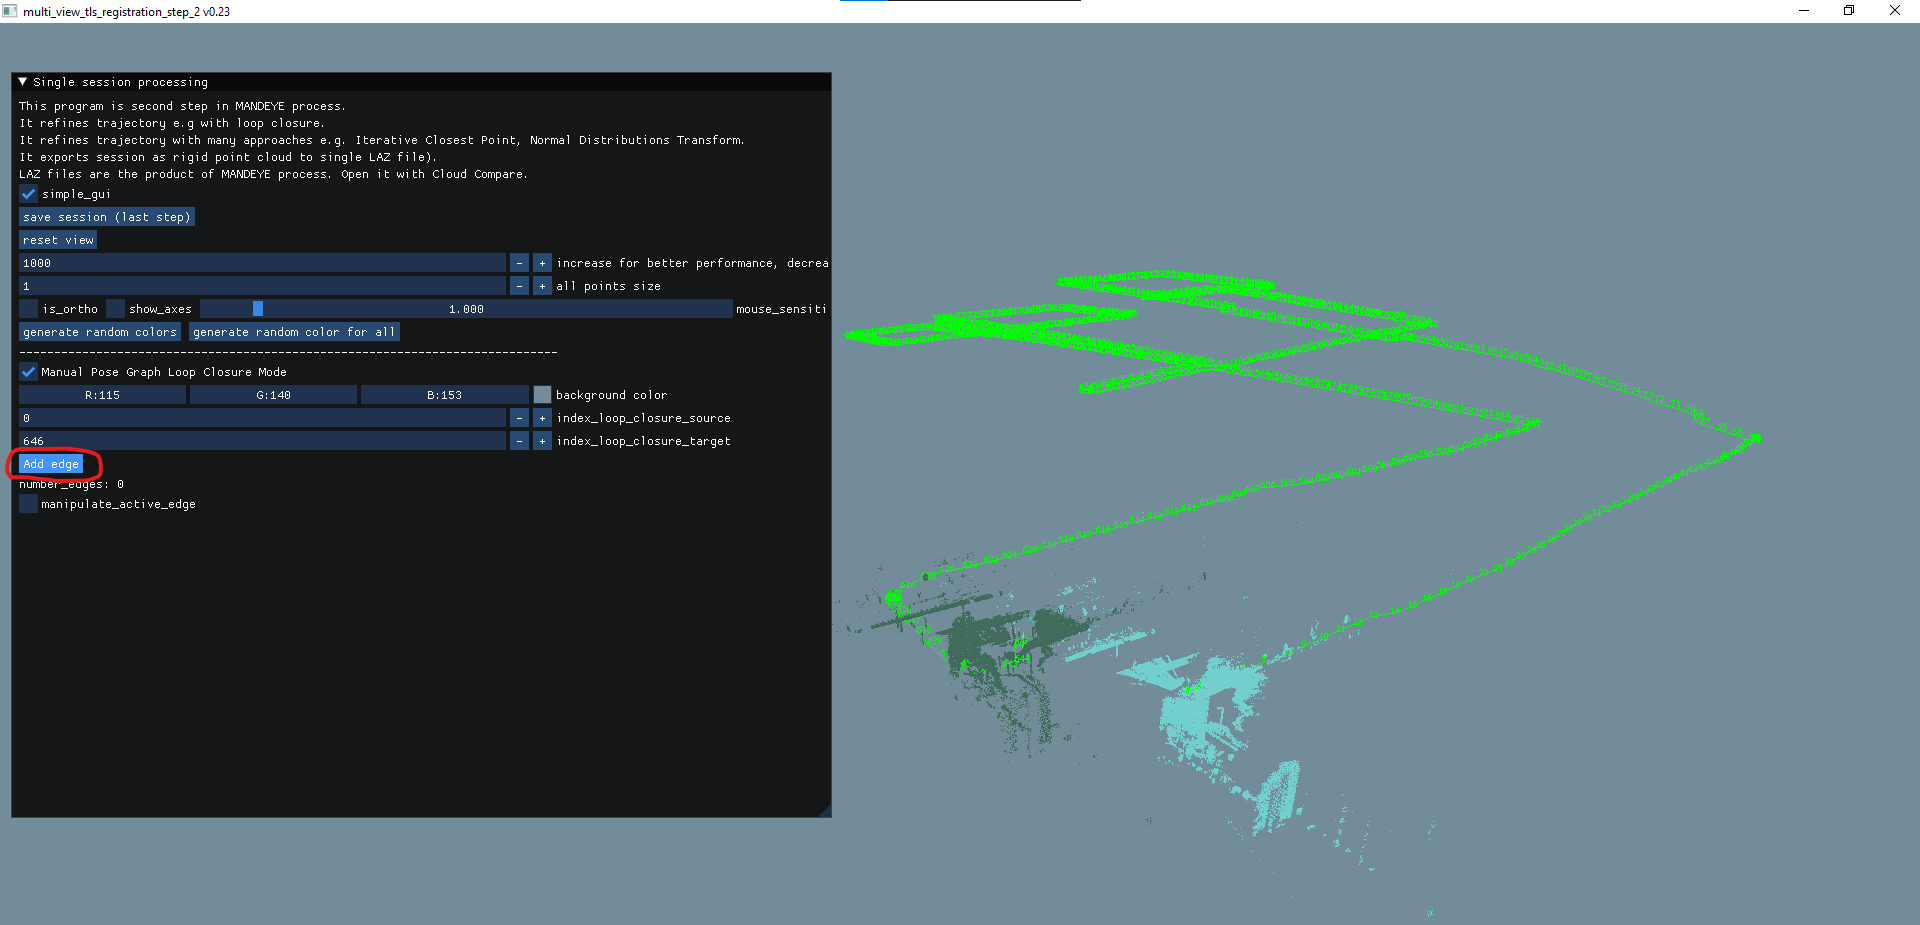
\includegraphics[width=\textwidth]{14.png}
	\caption{Turn on manual loop closing mode and choose two different scans that are not close enough. Add edge.}
	\label{fig:14}
\end{figure}


\begin{figure}
	\centering
	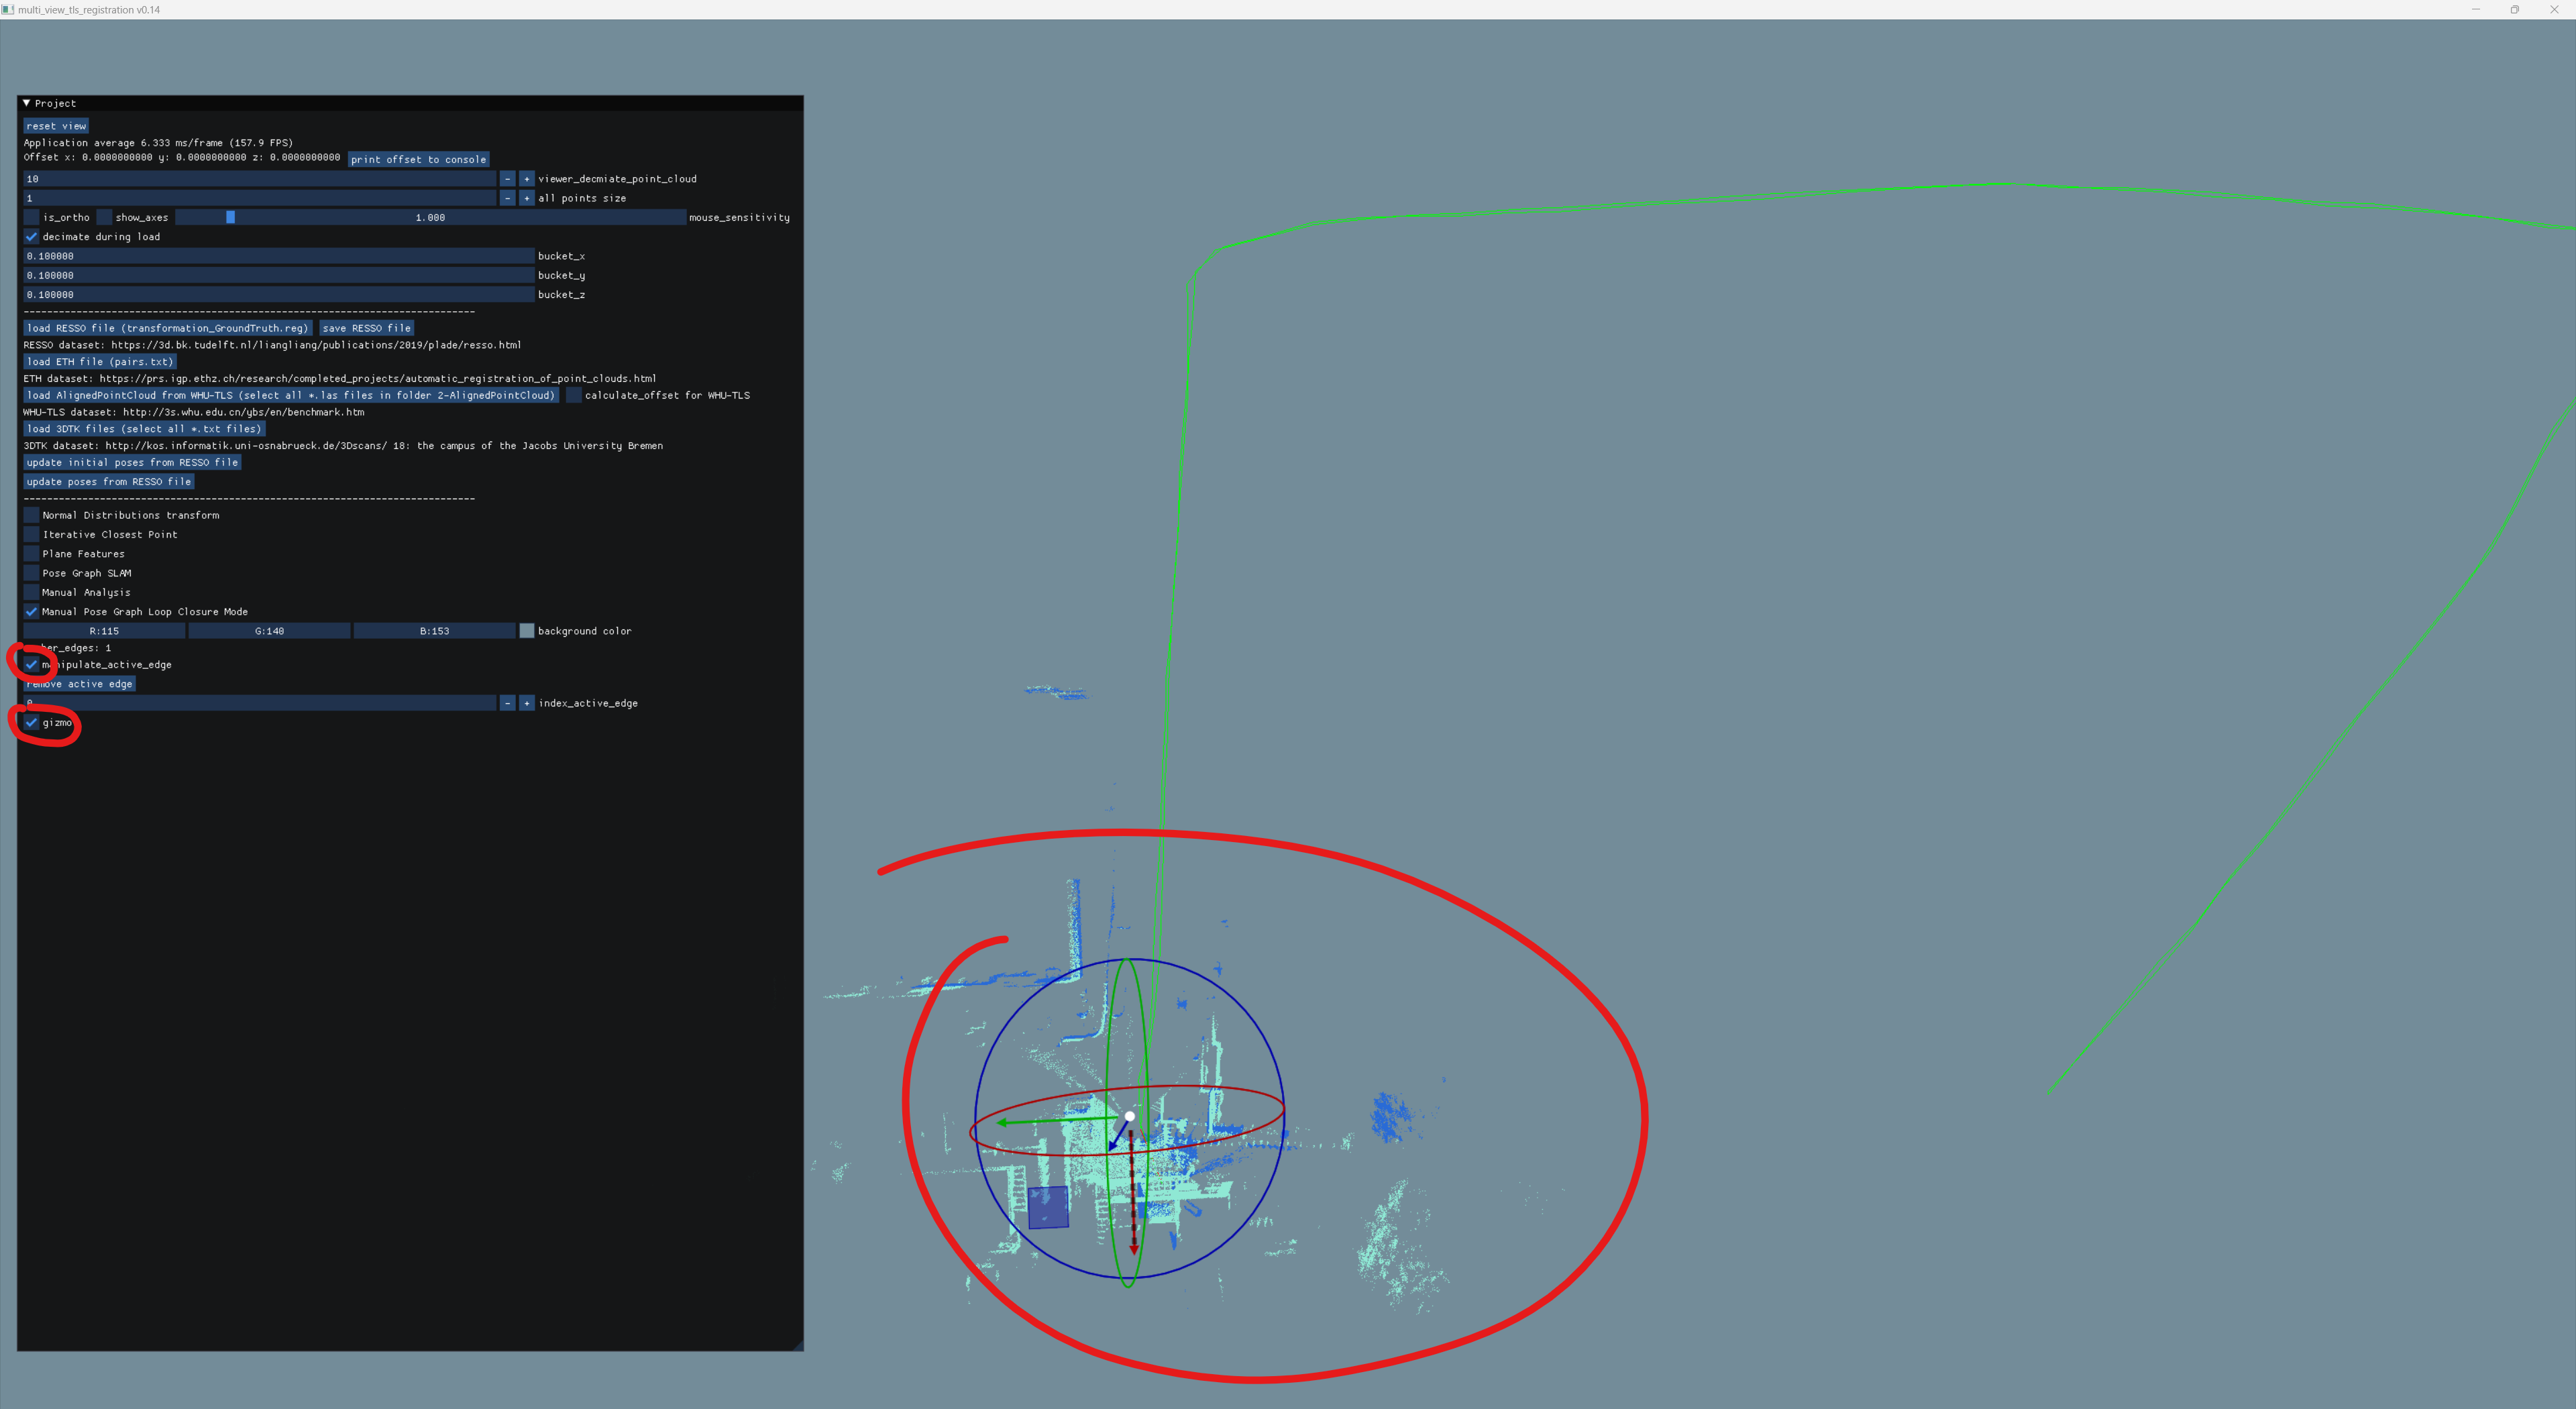
\includegraphics[width=\textwidth]{15.png}
	\caption{Turn on manipulate active edge, turn on gizmo and align scan to scan manually.}
	\label{fig:15}
\end{figure}

\begin{figure}
	\centering
	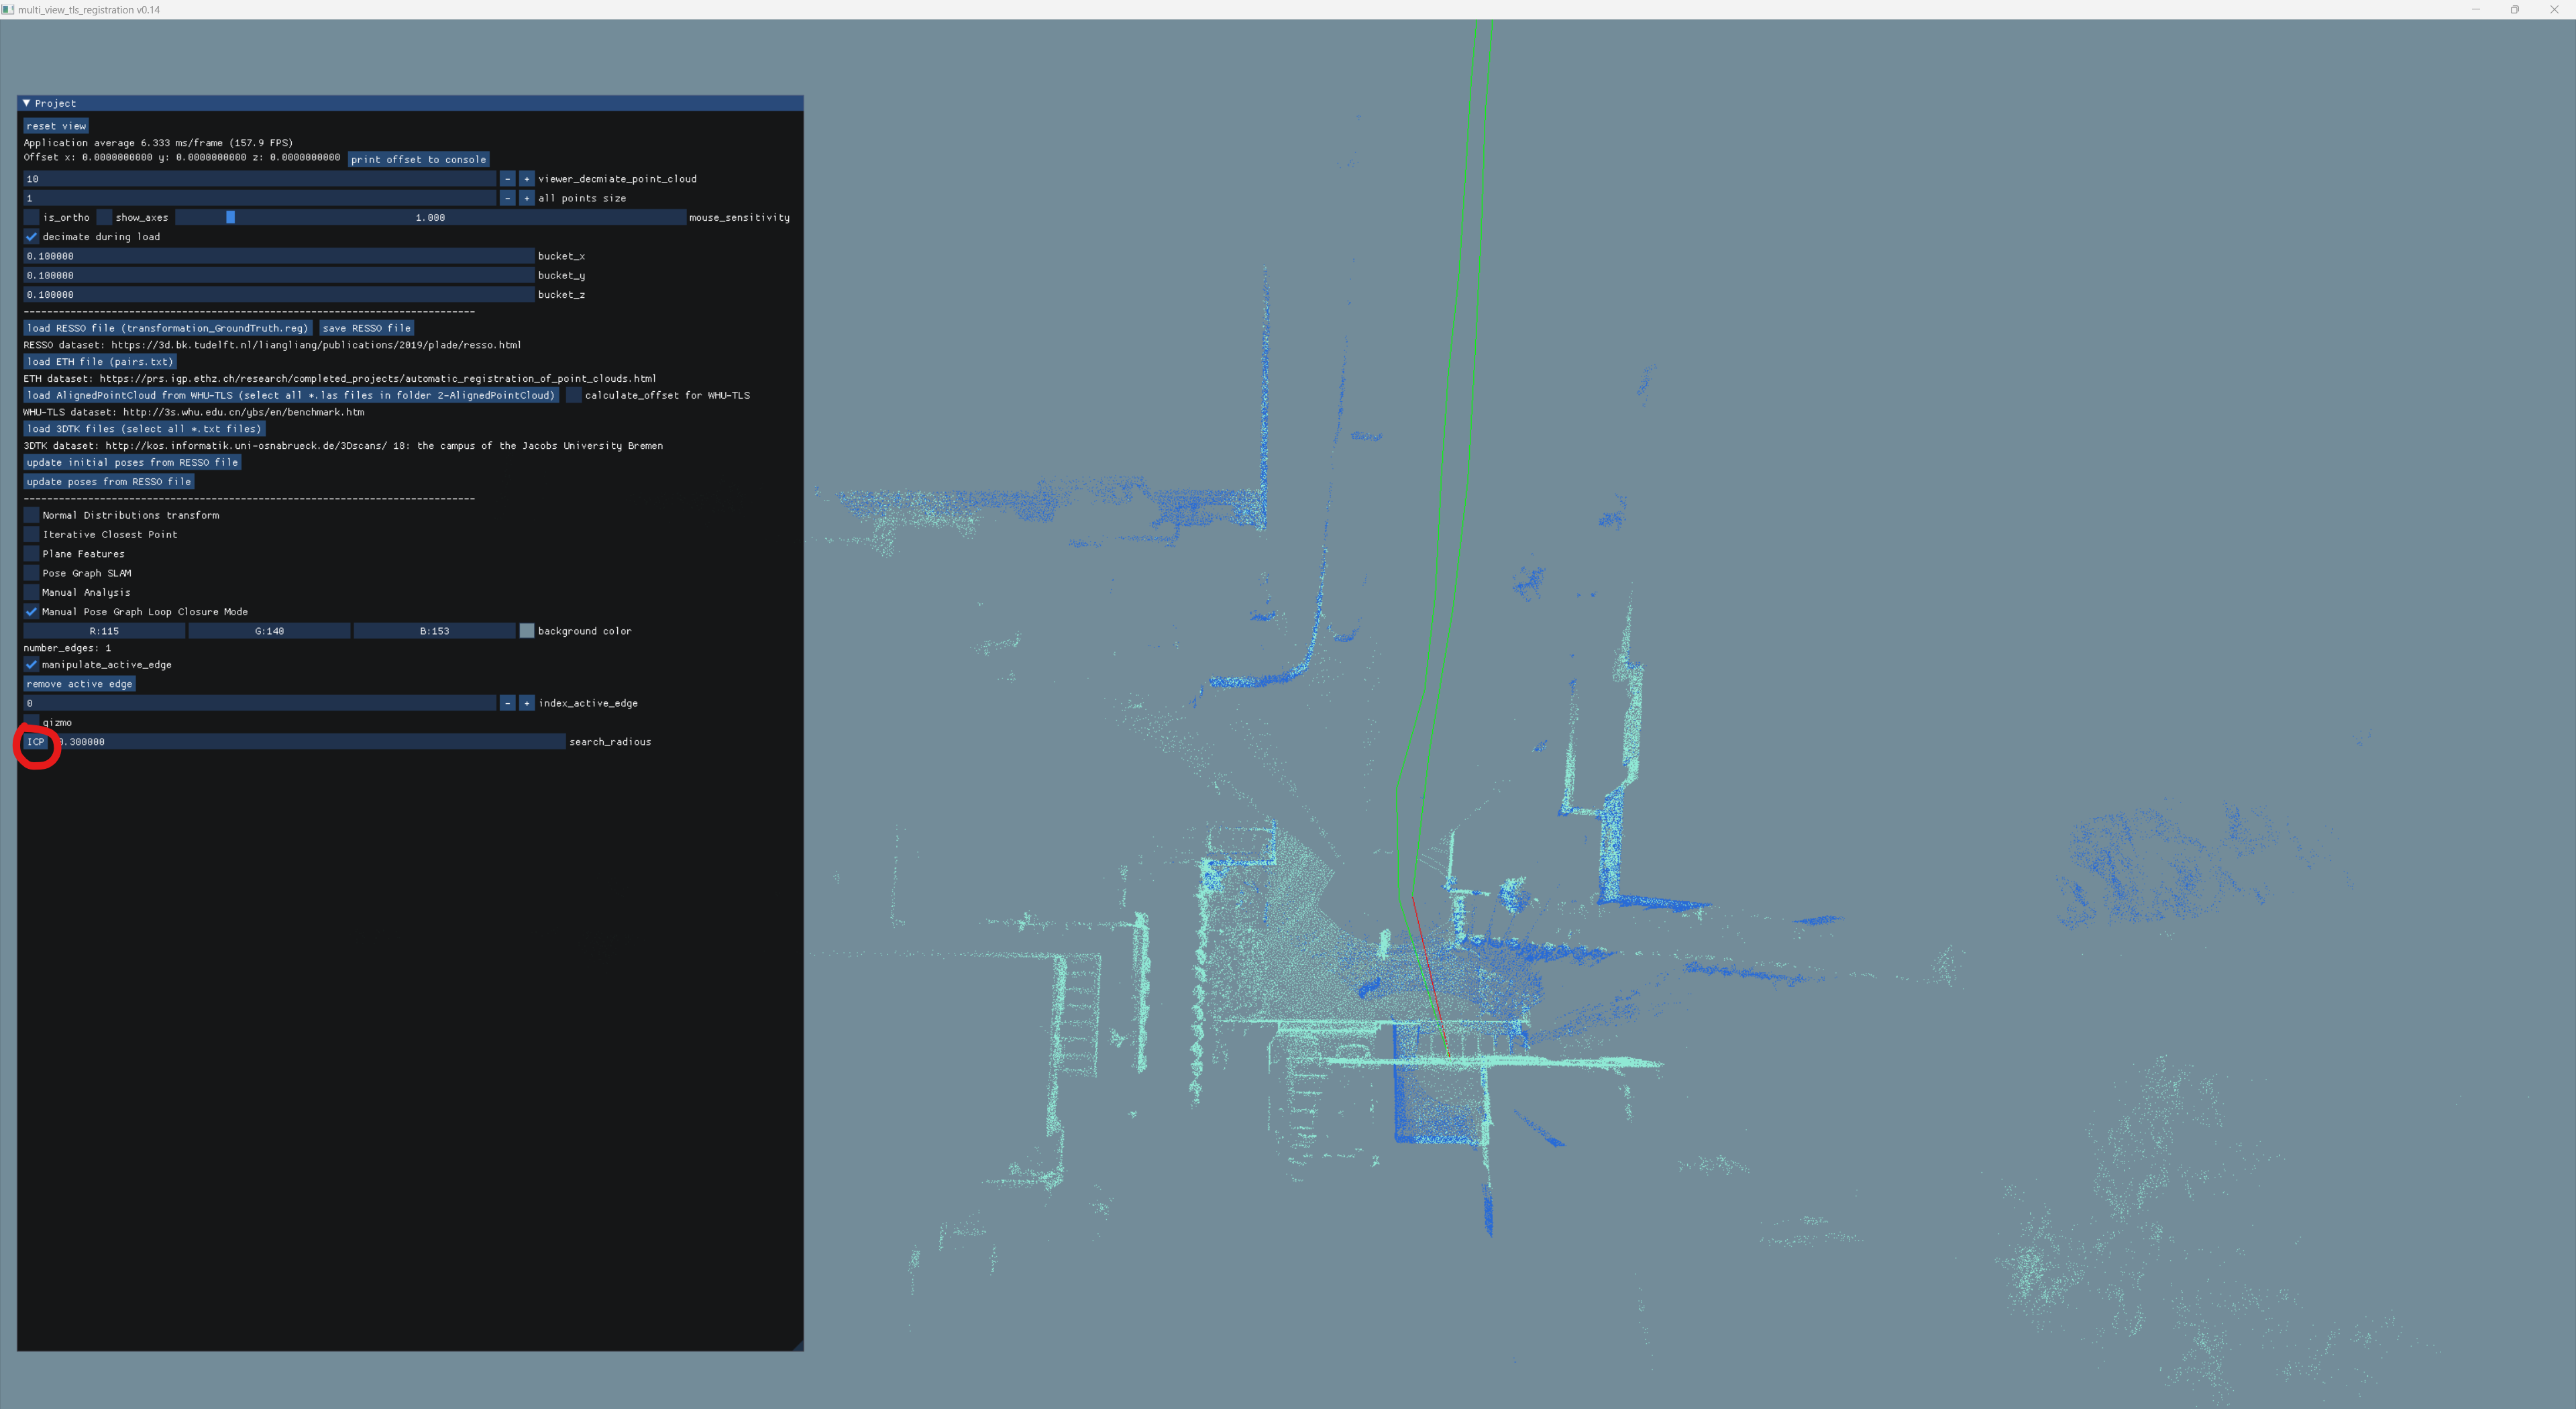
\includegraphics[width=\textwidth]{16.png}
	\caption{Once You are not capable align more accurate, then turn off gizmo and use ICP.}
	\label{fig:16}
\end{figure}

\begin{figure}
	\centering
	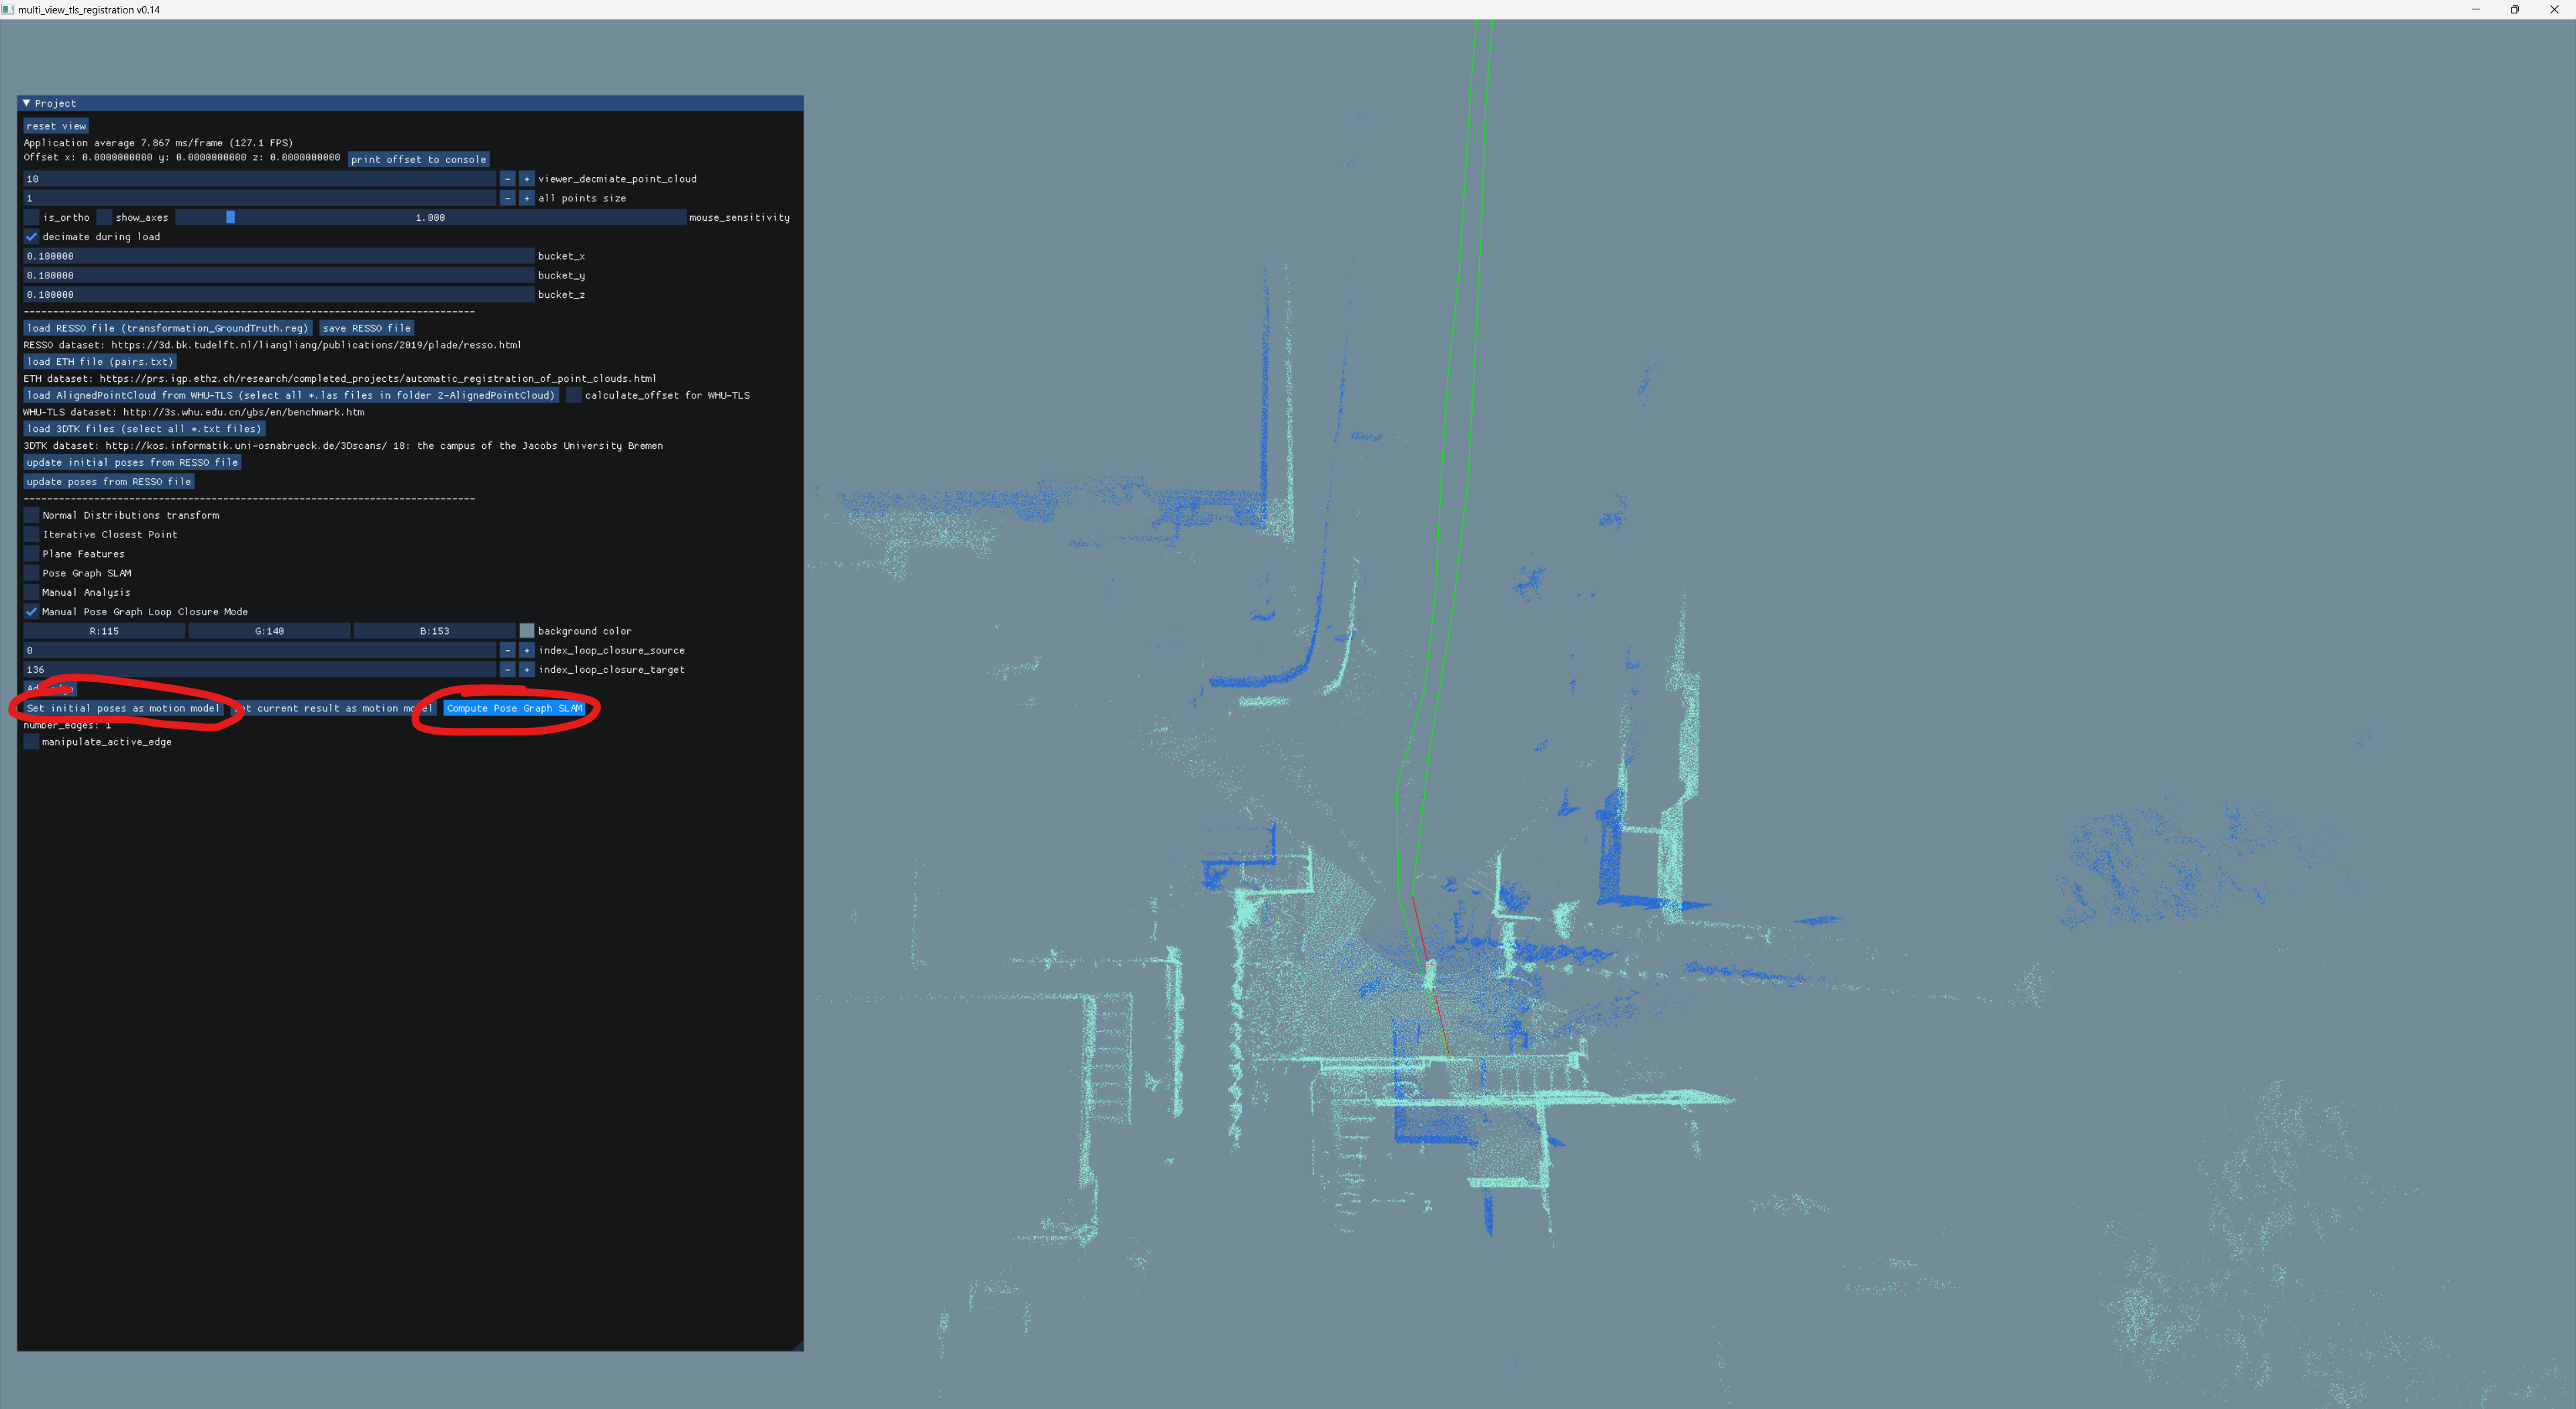
\includegraphics[width=\textwidth]{17.png}
	\caption{Turn off manipulate active edge, set initial poses as motion model, compute pose graph SLAM.}
	\label{fig:17}
\end{figure}

\begin{figure}
	\centering
	\includegraphics[width=\textwidth]{18.png}
	\caption{Turn off manual loop closing mode and inspect if everything ok, if not continue by choosing another pair of scans, refining them and repeat computation of the pose graph SLAM.}
	\label{fig:18}
\end{figure}

\begin{figure}
	\centering
	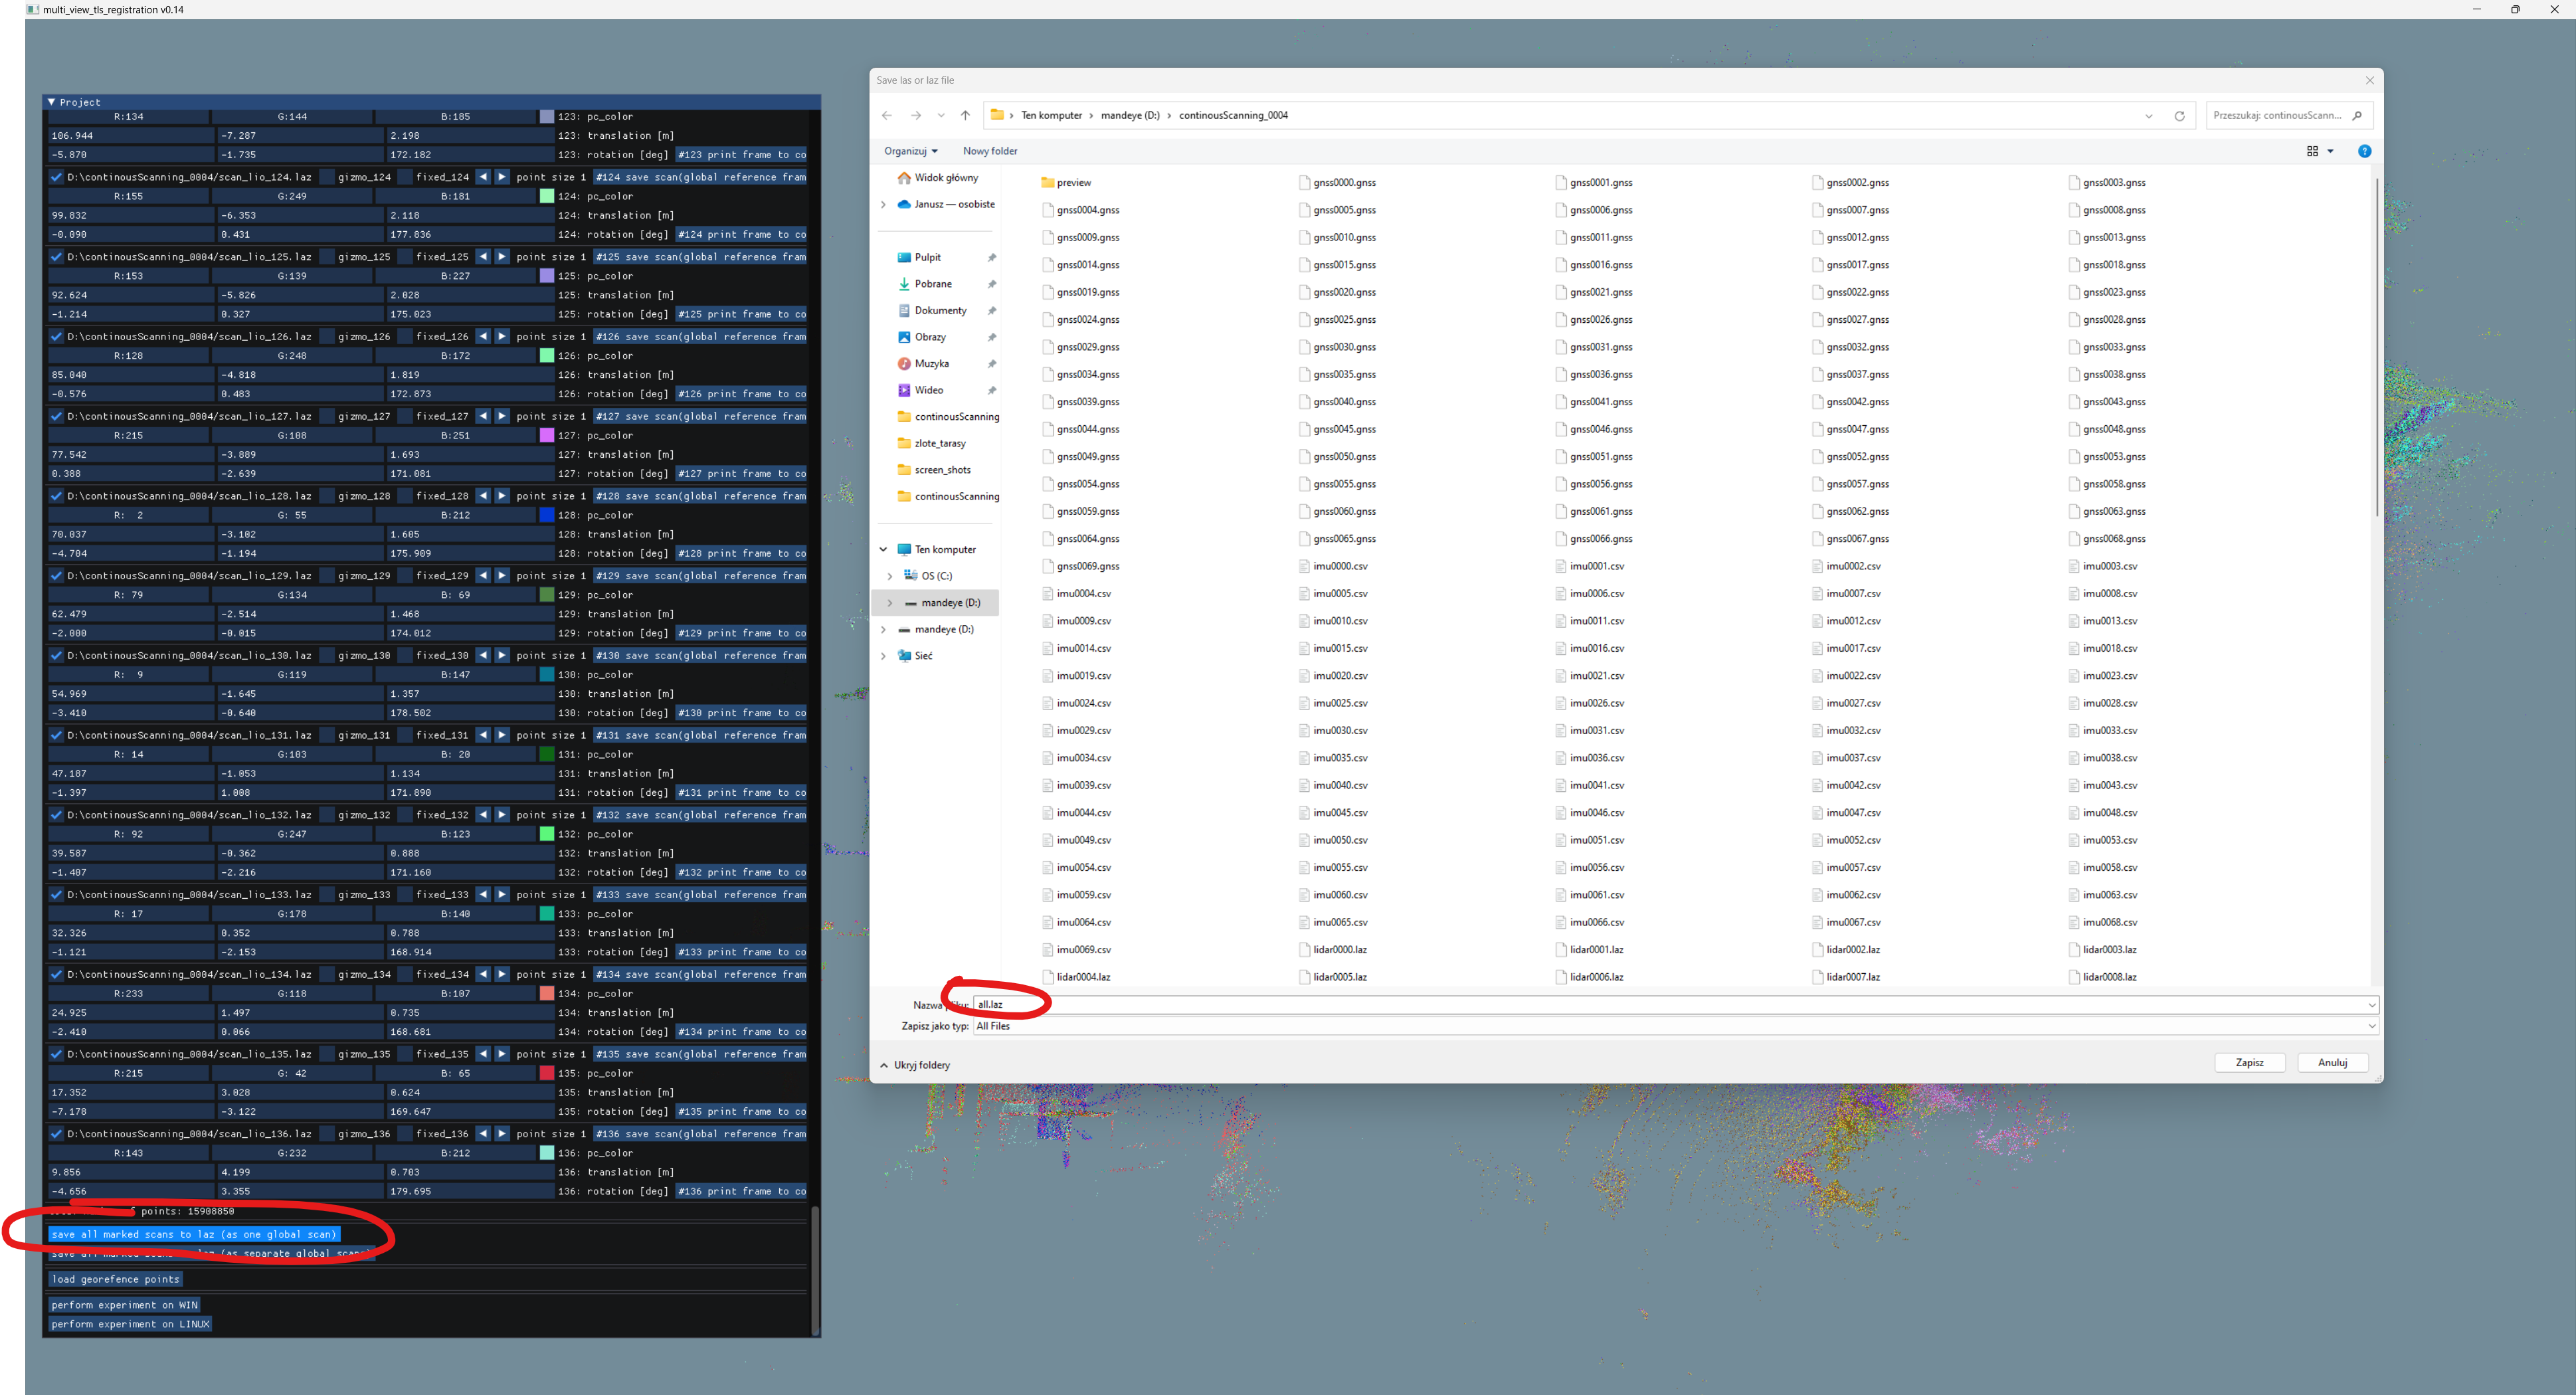
\includegraphics[width=\textwidth]{19.png}
	\caption{Ones the job is thon export data to *.laz. This is Your map that can be loaded by e.g. \href{https://www.cloudcompare.org/}{CloudCompare}.}
	\label{fig:19}
\end{figure}